%%
%% This is file `sample-sigplan.tex',
%% generated with the docstrip utility.
%%
%% The original source files were:
%%
%% samples.dtx  (with options: `sigplan')
%% 
%% IMPORTANT NOTICE:
%% 
%% For the copyright see the source file.
%% 
%% Any modified versions of this file must be renamed
%% with new filenames distinct from sample-sigplan.tex.
%% 
%% For distribution of the original source see the terms
%% for copying and modification in the file samples.dtx.
%% 
%% This generated file may be distributed as long as the
%% original source files, as listed above, are part of the
%% same distribution. (The sources need not necessarily be
%% in the same archive or directory.)
%%
%%
%% Commands for TeXCount
%TC:macro \cite [option:text,text]
%TC:macro \citep [option:text,text]
%TC:macro \citet [option:text,text]
%TC:envir table 0 1
%TC:envir table* 0 1
%TC:envir tabular [ignore] word
%TC:envir displaymath 0 word
%TC:envir math 0 word
%TC:envir comment 0 0
%%
%%
%% The first command in your LaTeX source must be the \documentclass command.
\documentclass[sigplan,anonymous,review]{acmart}

%%
%% \BibTeX command to typeset BibTeX logo in the docs
\AtBeginDocument{%
  \providecommand\BibTeX{{%
    Bib\TeX}}}

%% Rights management information.  This information is sent to you
%% when you complete the rights form.  These commands have SAMPLE
%% values in them; it is your responsibility as an author to replace
%% the commands and values with those provided to you when you
%% complete the rights form.
\setcopyright{acmcopyright}
\copyrightyear{2018}
\acmYear{2018}
\acmDOI{XXXXXXX.XXXXXXX}

%% These commands are for a PROCEEDINGS abstract or paper.
\acmConference[Conference acronym 'XX]{Make sure to enter the correct
  conference title from your rights confirmation emai}{June 03--05,
  2018}{Woodstock, NY}
\acmPrice{15.00}
\acmISBN{978-1-4503-XXXX-X/18/06}


%%
%% Submission ID.
%% Use this when submitting an article to a sponsored event. You'll
%% receive a unique submission ID from the organizers
%% of the event, and this ID should be used as the parameter to this command.
%%\acmSubmissionID{123-A56-BU3}

%%
%% For managing citations, it is recommended to use bibliography
%% files in BibTeX format.
%%
%% You can then either use BibTeX with the ACM-Reference-Format style,
%% or BibLaTeX with the acmnumeric or acmauthoryear sytles, that include
%% support for advanced citation of software artefact from the
%% biblatex-software package, also separately available on CTAN.
%%
%% Look at the sample-*-biblatex.tex files for templates showcasing
%% the biblatex styles.
%%

%%
%% The majority of ACM publications use numbered citations and
%% references.  The command \citestyle{authoryear} switches to the
%% "author year" style.
%%
%% If you are preparing content for an event
%% sponsored by ACM SIGGRAPH, you must use the "author year" style of
%% citations and references.
%% Uncommenting
%% the next command will enable that style.
%%\citestyle{acmauthoryear}

\usepackage{booktabs, multirow} % for borders and merged ranges
\usepackage{soul}% for underlines
\usepackage{comment}
\usepackage{wrapfig}
%A set of custom commands that are used for my personal latex style
%Created: Feb 2020
%Updated: July 2020
\usepackage{listings}

\newcommand{\defn}[1]{\textbf{#1}} %definitions are bold
\newcommand{\jnote}[1]{\textcolor{blue}{Justin: #1\\}} %a note from Justin
\newcommand{\rnote}[1]{\textcolor{orange}{Ron: #1\\}} %a note from Ron
\newcommand{\pnote}[1]{\textcolor{purple}{Peyton: #1\\}} %a note from Peyton
\newcommand{\todo}[1]{\textcolor{red}{TODO: #1\\}} %a todo note

\definecolor{tangerine}{RGB}{245,166,35} %comments, primary color
\definecolor{blueSeaFoam}{RGB}{80,227,194}
\definecolor{liteGreen}{RGB}{184,233,134 }
\definecolor{royalBlue}{RGB}{74,144,226} %keywords
\definecolor{amaranth}{rgb}{0.9, 0.17, 0.31} %special keywords
\definecolor{lavender}{rgb}{0.71, 0.49, 0.86}

\lstdefinestyle{mystyle}{
    backgroundcolor=\color{white},   
    commentstyle=\color{tangerine},
    keywordstyle=\color{royalBlue},
    identifierstyle=\color{black},
    numberstyle=\tiny\color{gray},
    basicstyle=\ttfamily\footnotesize,
    breakatwhitespace=false,         
    breaklines=true,                 
    captionpos=b,                    
    keepspaces=true,                 
    numbers=left,                    
    numbersep=5pt,                  
    showspaces=false,                
    showstringspaces=false,
    showtabs=false,                  
    tabsize=2,
    frame=lines,
    %just for Chisel
    emph={Module, IO, Input, Output, UInt, Bool, Wire, Vec, before, after, extend, in, register, insert, apply, Pointcutter, AfterToken},
    emphstyle=\color{amaranth}
}

\lstset{style=mystyle}


%% Algorithms
\usepackage{algorithm}
\usepackage{algorithmic}
% \usepackage{algorithm2e}
% \RestyleAlgo{ruled}


%%
%% end of the preamble, start of the body of the document source.
\begin{document}

%%
%% The "title" command has an optional parameter,
%% allowing the author to define a "short title" to be used in page headers.
\title{Feature-Oriented Construction of Finite State Machines}

%%
%% The "author" command and its associated commands are used to define
%% the authors and their affiliations.
%% Of note is the shared affiliation of the first two authors, and the
%% "authornote" and "authornotemark" commands
%% used to denote shared contribution to the research.
\author{Ben Trovato}
\authornote{Both authors contributed equally to this research.}
\email{trovato@corporation.com}
\orcid{1234-5678-9012}
\author{G.K.M. Tobin}
\authornotemark[1]
\email{webmaster@marysville-ohio.com}
\affiliation{%
  \institution{Institute for Clarity in Documentation}
  \streetaddress{P.O. Box 1212}
  \city{Dublin}
  \state{Ohio}
  \country{USA}
  \postcode{43017-6221}
}

\author{Lars Th{\o}rv{\"a}ld}
\affiliation{%
  \institution{The Th{\o}rv{\"a}ld Group}
  \streetaddress{1 Th{\o}rv{\"a}ld Circle}
  \city{Hekla}
  \country{Iceland}}
\email{larst@affiliation.org}

\author{Valerie B\'eranger}
\affiliation{%
  \institution{Inria Paris-Rocquencourt}
  \city{Rocquencourt}
  \country{France}
}

\author{Aparna Patel}
\affiliation{%
 \institution{Rajiv Gandhi University}
 \streetaddress{Rono-Hills}
 \city{Doimukh}
 \state{Arunachal Pradesh}
 \country{India}}

\author{Huifen Chan}
\affiliation{%
  \institution{Tsinghua University}
  \streetaddress{30 Shuangqing Rd}
  \city{Haidian Qu}
  \state{Beijing Shi}
  \country{China}}

\author{Charles Palmer}
\affiliation{%
  \institution{Palmer Research Laboratories}
  \streetaddress{8600 Datapoint Drive}
  \city{San Antonio}
  \state{Texas}
  \country{USA}
  \postcode{78229}}
\email{cpalmer@prl.com}

\author{John Smith}
\affiliation{%
  \institution{The Th{\o}rv{\"a}ld Group}
  \streetaddress{1 Th{\o}rv{\"a}ld Circle}
  \city{Hekla}
  \country{Iceland}}
\email{jsmith@affiliation.org}

\author{Julius P. Kumquat}
\affiliation{%
  \institution{The Kumquat Consortium}
  \city{New York}
  \country{USA}}
\email{jpkumquat@consortium.net}

%%
%% By default, the full list of authors will be used in the page
%% headers. Often, this list is too long, and will overlap
%% other information printed in the page headers. This command allows
%% the author to define a more concise list
%% of authors' names for this purpose.
\renewcommand{\shortauthors}{Trovato et al.}

%%
%% The abstract is a short summary of the work to be presented in the
%% article.
\begin{abstract}
We investigate the generation of complex, featureful finite-state machines from relatively simpler ones using two constructs.  The first, inspired by aspect-oriented programming, applies incremental changes to the states and edges of a finite-state machine to alter and customize its behavior in response to features of interest.   This allows efficient specification and generation of numerous designs, each containing only those features of interest for a particular application.

The second construct couples the behavior of multiple finite machines into a single machine that processes its inputs simultaneously.  While this is formally the concatenation of regular languages, we present a \emph{cross-product} algorithm that allows the resulting design to process its wider inputs in lock-step.  This is necessary for the proper timing of actions taken by the resulting machine. 

Each construct is illustrated and results are presented using a simple example:  a vending machine and the game of Nim, respectively.  We then apply the constructs in concert to generate a coherent, $n$-way multiprocessor cache from a much simpler specification.

We show that our approach can generate designs that are exponentially large in the size of their specifications.  In addition to that significant design leverage, the resulting finite-state machines enjoy all the closure properties and proof opportunities for regular languages.
\end{abstract}

%%
%% The code below is generated by the tool at http://dl.acm.org/ccs.cfm.
%% Please copy and paste the code instead of the example below.
%%
\begin{CCSXML}
<ccs2012>
<concept>
<concept_id>10011007.10011006.10011041.10011047</concept_id>
<concept_desc>Software and its engineering~Source code generation</concept_desc>
<concept_significance>500</concept_significance>
</concept>
<concept>
<concept_id>10010583.10010682.10010689</concept_id>
<concept_desc>Hardware~Hardware description languages and compilation</concept_desc>
<concept_significance>500</concept_significance>
</concept>
</ccs2012>
\end{CCSXML}

\ccsdesc[500]{Software and its engineering~Source code generation}
\ccsdesc[500]{Hardware~Hardware description languages and compilation}

%%
%% Keywords. The author(s) should pick words that accurately describe
%% the work being presented. Separate the keywords with commas.
\keywords{feature-oriented programming, finite state machines, generative programming, hardware generation}
%% A "teaser" image appears between the author and affiliation
%% information and the body of the document, and typically spans the
%% page.

%%
%% This command processes the author and affiliation and title
%% information and builds the first part of the formatted document.
\maketitle

\section{Introduction}

The advent of hardware-generation languages~\cite{chisel:article} has promoted the adoption of techniques and abstractions by hardware designers that were previously available only to software systems and their designers. Hardware-characterization languages such as VHDL~\cite{vhdl} and Verilog~\cite{verilog} describe the components and interconnections of hardware circuit elements, much like HTML describes the components and references of a web page. While those languages provide some abstractions (such as arithmetic operations and restrictive macros), the paradigms and practices used widely in successful software engineering efforts are largely unavailable.

By contrast, hardware-generation approaches allow a designer to write a program whose execution generates the hardware design. The program can be authored using para\-digms that promote efficiency, reuse, rigorous testing, and clarity of expression. Our work in this paper builds on the hardware-generation language Chisel~\cite{chisel:book}, which is in turn built on Scala~\cite{scala-overview-tech-report}. Chisel is a Scala-embedded domain specific language and libraries that generate Verilog when a Chisel program is executed.

A simple and recent example showing the advantages of hardware generation over characterization concerns an adder~\cite{Deters:adder}. Using VHDL, a hardware designer can request that an adder circuit be optimized for either for delay (carry lookahead) or for area (carry propagate). Using Chisel, an adder can be specified that combines both forms of carry computation, to meet a timing or area constraint while otherwise optimized in the other dimension.

Chisel has also proven itself robust in pedagogy and industry, serving as the basis for courses in digital logic~\cite{vlsicourse} and serving as a platform for describing RISC-V systems~\cite{chisel:riscv}.  Our long-term goal is to develop a feature-oriented characterization of RISC-V~\cite{riscv}.  Here we focus on a specific, more modest construct used in hardware designs.

In this paper, we consider a feature-oriented approach to generating hardware, specifically \emph{finite state machines} (FSMs). A given feature can affect multiple regions of an FSM. For example, the cache system  we consider in Section~\ref{sec:cache} could use write-back or write-through in response to a store operation. Expressed as a feature, write-back affects both the store operation (marking the line dirty) and the fetch operation (causing dirty lines to be written to the backing store on eviction). Aspect-oriented programming (AOP)~\cite{gregor:97} is a paradigm well suited to expression of cross-cutting concerns that affect multiple regions of software systems. For example, AspectJ~\cite{aspectj} allows expression of advice that is applied at prescribed join points of a software system written in Java. While our thinking is aspectual in terms of formulating a feature-oriented approach to finite state machines, we are fortunate that hardware generation languages such as Chisel suffice to express the requisite transformations and code generation:  no new language is needed.

In Section~\ref{sec:prior} we summarize feature-oriented approaches for software systems and other inspirations for our work. As compared with monolithic designs, feature-oriented systems omit unnecessary code, resulting in smaller footprint and higher throughput.
Sections~\ref{sec:decomp} and~\ref{sec:formal} describe a feature-oriented approach for generating finite state machines using two complementary techniques. We illustrate those techniques separately on the examples of a vending machine (Section~\ref{sec:vend}) and the game of Nim (Section~\ref{sec:nim}). In Section~\ref{sec:cache}, the techniques are then applied in concert to generate a multiprocessor cache with a simple coherence protocol.

\section{Prior work and motivation}\label{sec:prior}

\subsection{Aspect-oriented programming}

Our work builds on a programming paradigm available in the software community that efficiently supports the expression and application of \emph{cross-cutting} concerns in a software system.  Aspect-Oriented Programming~(AOP)~\cite{gregor:97} and its realization in systems such as AspectJ~\cite{aspectj} allow developers to express ideas in a software system that affect multiple components of that system in support of a common idea or feature. A commonly cited example is the implementation of a logging feature, so that every method when called and prior to returning logs those events to some output stream. Absent an AOP approach, a developer is faced with the following difficulties:
\begin{itemize}
    \item Implementation of the feature would require modifying every method at its entry and every possible exit so that it emitted the proper log messages.  This is both tedious and error-prone, especially if methods can exit due to unforeseen actions such as exceptions.
    \item Removing the feature, should it no longer be needed, is also tedious and error-prone.
    \item Placing the feature under some kind of conditional execution offers some relief, but
    \begin{itemize}
        \item The conditions themselves incur execution time and the logging code occupies code space.
        \item Subsequent modifications to the system must be mindful to include properly the logging actions.
    \end{itemize}
\end{itemize}
Macro processors can achieve the proper effect, namely including the code only when it is desired.  However, it is still incumbent on developers to remember to call the macros at the proper points in a program.

AOP is the perfect solution to this and similar problems, because a developer can specify that at \emph{every} method entry and exit (other than the method that does the logging), a segment of code should be inserted to accomplish the appropriate logging.  If the logging is no longer desired, the associated aspect is simply omitted when building the system.  In this way, both originally and upon modification, all methods' entries and exits are properly logged.

\subsection{Feature-oriented programming}\label{sec:priorfop}
\jnote{Since this conference is asking specifically for FOP, do we need this much background detail? Would it be better to focus on other hardware construction?}
Feature-Oriented Programming~(FOP)~\cite{prehofer1997feature} builds on this idea by expressing features in an aspectual manner. A feature is essentially a recipe for rewriting a software system to implement the feature. The common example given for this paradigm is that of a \emph{cache}, say in a web browser.  Where the browser would normally issue a request to a website on behalf of a given URL (which could take some time), the cache feature would first check if the browser had recently fetched that URL, satisfying the request with the cached information. Implementation of this feature requires storage to hold previously fetched information, code to manage that storage, and a rewrite of the base system to cause the cache to be consulted prior to issuing the web request. Expressed aspectually, a cache could be imposed throughout the browser, in any situation where such a web request could be made.

The feature on its own is insufficient to realize any benefits. The software system must be written in such a way to accept the feature. As more features are conceived and implemented, the base system and any extant features may require revision. In the end, a system is obtained where orthogonal features compose effortlessly, in any combination, to realize a desired subset of all possible features.

This approach to creating featureful systems has the empirical advantages described below. This approach has also been attractive for managing product lines in which features evolve over time, affecting not only the base system but also other features~\cite{10.1145/2897695.2897701}.

An example that has been treated with this approach is the CORBA~\cite{CORBA:00} Event Channel~\cite{CORBAService:02a}. The standard implementation is \emph{monolithic}, offering all possible features in all allowable combinations.    
When expressed in terms of composable features, configurations of interest could be generated that contained only those desired features (and their dependencies).

\rnote{Ron talks about the efficiency results. if room, we can provide a graph.  must be anonymous}

In this paper, we consider applying a feature-oriented approach to specifying hardware designs, namely finite-state machines.
The resulting designs enjoy the same benefits as the software systems we describe above:
\begin{itemize}
    \item Smaller footprint results by including only those features of interest.
    \item The clock rate of the resulting systems is determined only by active features:  logic related to inactive features is completely absent from the resulting designs.
\end{itemize}

\subsection{Generative programming}\label{sec:priorgen}
Our approach to building FSMs is generative~\cite{10.1007/11527800_24} in the following ways:
\begin{itemize}
    \item A Chisel program generates a hardware specification by its execution.  Thus, Chisel allows us to generate FSMs without the burden of developing a specific AOP language for our work.
    \item Our FOP approach generates an FSM that incorporates only those features of interest.  This is demonstrated by the vending machine example of Section~\ref{sec:vend}, in which the construction of even the simplest, base machine is driven automatically by allowable currency values.  If there are $k$ orthogonal features in a system, each present or not, then our approach allows the generation of~$O(2^{k})$ potential FSMs using~$O(k)$ space to express those features.
    \item As demonstrated in Section~\ref{sec:nim}, a given feature may benefit in our approach from factoring it into simpler FSMs that are insufficient on their own, but whose \emph{cross product} achieves a desired feature.  Here is a specification that takes~$O(k)$ space, can generate an FSM of size~$O(2^{k})$.
\end{itemize}
Our generative approach to building FSMs thus has the following advantages:
\begin{itemize}
    \item The realization of very large FSMs can be achieved correctly by construction.
    \item The resulting FSMs contain only those features of interest and their dependencies.
    \item By limiting our work to FSMs, many properties of the resulting systems can be proven.  We discuss this next.
\end{itemize}
\rnote{check that we use FSM and finite-state machine properly throughout}
  
\subsection{Decidability}\label{sec:decide}

The theory of regular languages and finite-state machines allows that questions related to properties of the behavior of such machines have definite and algorithmically obtained answers~\cite{sipser}. For example, consider a feature that is intended to \emph{extend} the behavior of a design, so that all previous inputs are allowed, but the feature introduces some other allowable inputs. For example, consider an FSM that scans characters to parse them as decimal numerals.  An extension might allow for hexadecimal numerals, if the input begins with ``0x''.  We would like to prove that the extended language is indeed a proper superset of the original language, which is possible for finite-state machines.

While beyond the scope of this paper, we aim to use \emph{timed automata}~\cite{10.1145/2518102} to reason about real-time properties of finite-state machines generated by our approach.\rnote{maybe move to future work}

\section{Generative FSM specifications}

We next illustrate our two mechanisms for generating designs.  The first uses aspect-oriented advice to incorporate features selectively into an FSM.  The second builds an FSM from the synchronous execution of smaller FSMs.

\begin{comment}
\rnote{rewrite or omit?} A \emph{feature} in our system is a collection of states, transitions, or a combination of both, that can be selectively added to a finite state machine. Features can be decomposed into cross-cutting concerns, independent finite state machines, or a combination of the both. To demonstrate feature decomposition, we model a vending machine and the game of Nim using finite state machines.
\end{comment}

\subsection{Automating feature inclusion: vending machine}\label{sec:vend}

As an example of a featureful design, we consider an FSM design for a vending machine.   A state in our design carries the necessary \emph{traits} to represent its role in the machine's operation:  the funds inserted and the potential products dispensed.  Our generative approach described below offers the following advantages over a monolithic design:
\begin{itemize}
    \item The simplest design becomes correct by construction, with states generated automatically based on currency values.  Introduction of a new value of coinage automatically creates the necessary additional states.
    \item Features of interest are easily applied based on states' traits.
\end{itemize}
For this example and the results we present, the features of interest are as follows:
\begin{description}
    \item[Add Currency] introduces a value of coinage.
    \item[Dispense Product] introduces the price of a vendible item.
    \item[Print Funds] display the total funds after each state change.
    \item[Insufficient Funds] advises the user to insert more money to buy a particular item.
    \item[Change Return] causes the machine to return inserted funds.
    \item[Peanut Warning] requests confirmation of purchase for items that contain peanuts.
    \item[Buy More] allows the user to continue purchasing items if funds remain in the machine.
\end{description}
The dependencies of these features are shown in Figure~\ref{fig:vmDependencies}, but this graph is not needed for construction:  the advice for a given feature is applicable only when its associated \emph{join points} exist in the FSM.  As is typical with aspect-oriented approaches, all advice is presented to the weaver (our runtime library for Chisel), and the aspects are continually applied until no changes occur.

For example, the advice for Add Currency of coinage $k$ specifies that for any state representing that $n$ cents have been inserted, a state representing $n+k$ cents must exist, with a transition from state~$n$ to state~$n+k$ based on the insertion of coinage $k$.   This advice fails to terminate if not capped by some upper bound on funds, which could be related to the most expensive product sold. Figure \ref{fig:vend1} shows one such machine. Applying a 5 cent feature up to 15 cents and a 10 cent gum figure correctly generates all the necessary states. 

As another example, consider the Buy More feature, which causes the machine to retain funds after a purchase and allow for subsequent purchases.  Without this feature, the machine would return excess funds after a single purchase.  The advice for this feature modifies every purchase to move to a state representing currently held funds.

A monolithic approach requires designers to specify all states and transitions for each feature subset, which is tedious and error-prone. With our approach, all states and transitions are obtained generatively and are correct by construction, if the advice for their creation is correct.

\begin{figure*}
    \centering
    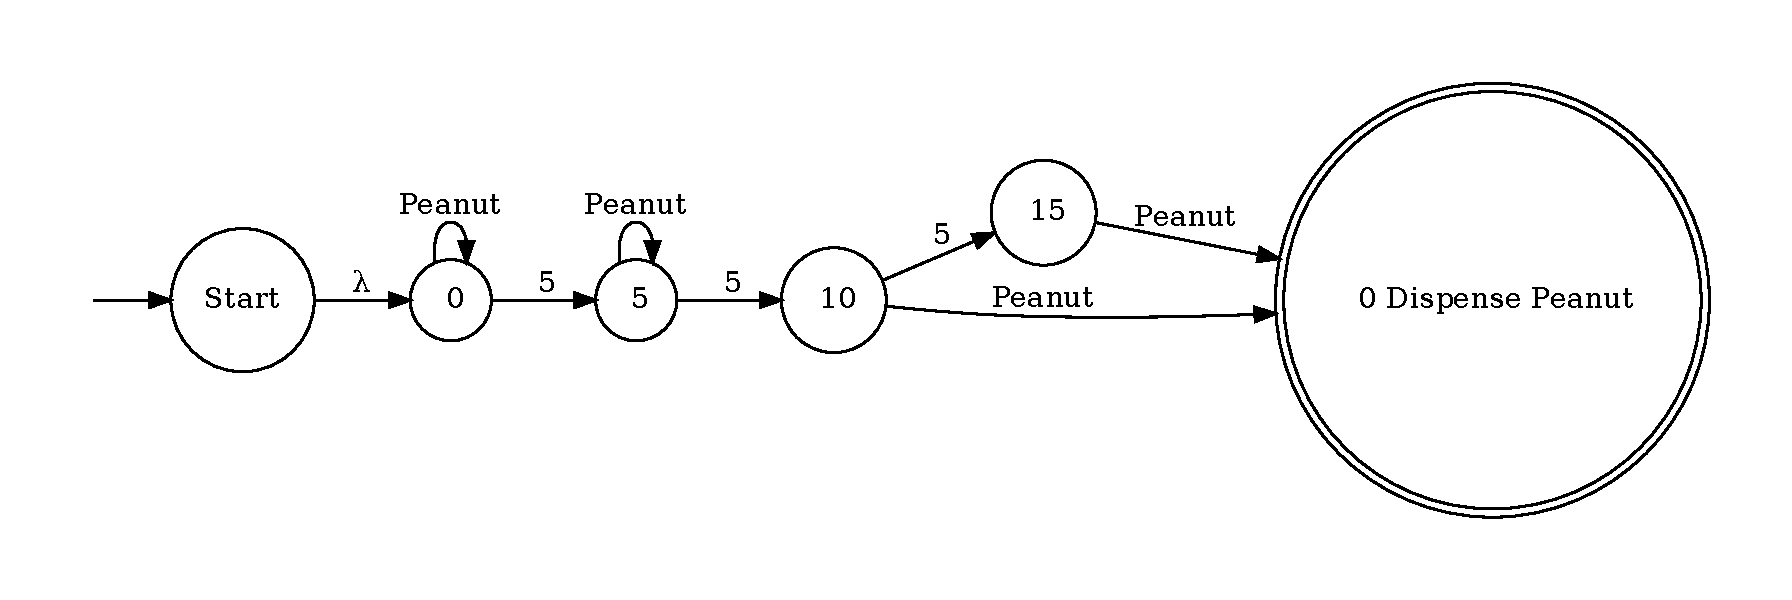
\includegraphics[width=0.7\textwidth]{figures/vend1.pdf}
    \caption{An example finite state machine that accepts 5 cent coins and dispenses 10 cent gum.}
    \label{fig:vend1}
\end{figure*}

\begin{figure}
    \centering
    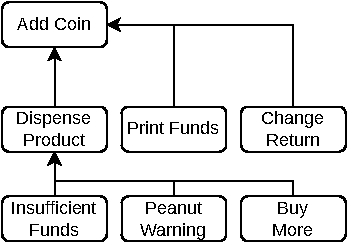
\includegraphics[width=0.5\linewidth]{figures/VendingMachine.pdf}
    \caption{Dependencies between vending machine features.}
    \label{fig:vmDependencies}
\end{figure}

\subsection{Composing machines: Nim}

Nim~\cite{nim} is a broad class of impartial mathematical strategy games, which traditionally involve multiple heaps of tokens (\textit{e.g.}, sticks) and two or more alternating players. The current player removes an allowable number of tokens from a subset of the heaps. The winner can be the player taking the last token, or (in the \textit{mis\`{e}re} version) that player loses.

While we initially approached this game with the ideas in Section~\ref{sec:vend}, states in this game represent the number of tokens present in each heap and the current player's turn.  Aspectual features should be additive, expanding the behavior of their targets, and while cross-cutting, they do not typically completely rewrite their targets.  With Nim, the machine is changed throughout by the addition of an additional player or heap.   However, we realized that construction of even the most basic game of Nim can be regarded as the composition or simultaneous operation of two simpler machines:   one that represents only the allowable subtractions of tokens in the heap and one that represents only the alternation of players.   By composing those and operating them in lock step, we can then generate an FSM that implements basic Nim.

Following is our decomposition of Nim:
\begin{description}
    \item[Heap Bounds] encodes the initial and winning number of tokens for each heap.
    \item[Legal Moves] encodes permissible combinations of adding and removing tokens from each heap.
    \item[Number of Players] specifies how many players alternate play in the game.
    \item[Win Type] specifies whether the game is mis\`{e}re play or normal play.
\end{description}
The dependencies of these features is shown in Figure~\ref{fig:nimDependencies}.  

\begin{figure}
    \centering
    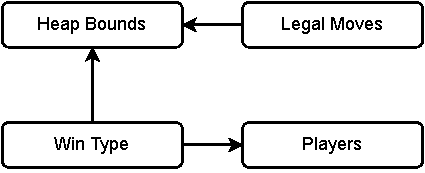
\includegraphics[width=0.5\linewidth]{figures/NimFeatures.pdf}
    \caption{Dependencies between Nim features.}
    \label{fig:nimDependencies}
\end{figure}

We consider a basic two-player (Figure~\ref{fig:nimPlayerFSM}) game using a single, subtractive heap of 5 tokens (Figure~\ref{fig:nimHeapFSM}).
A winner can be declared when:
\begin{itemize}
    \item In Figure~\ref{fig:nimPlayerFSM}, the players truly alternate.  For example, the sequence ABA can lead to an accept, but the sequence AAB cannot.
    \item In Figure~\ref{fig:nimHeapFSM}, an accepting sequence is 212.
\end{itemize}
Formally, in the theory of regular languages, we seek the \emph{concatenation} of the languages of these two machines.   Given the sequence ABA and 212, each accepted by its respective machine, the concatenation ABA212 is a string in the concatenation of the two languages.  While this correctly represents the sequence of inputs that causes somebody to win, the timing of actions associated with transitions in the two machines does not coincide properly.  For example, it is not possible in the concatenation to determine \emph{who} won the game when the second machine accepts. 

\begin{figure}
    \centering
    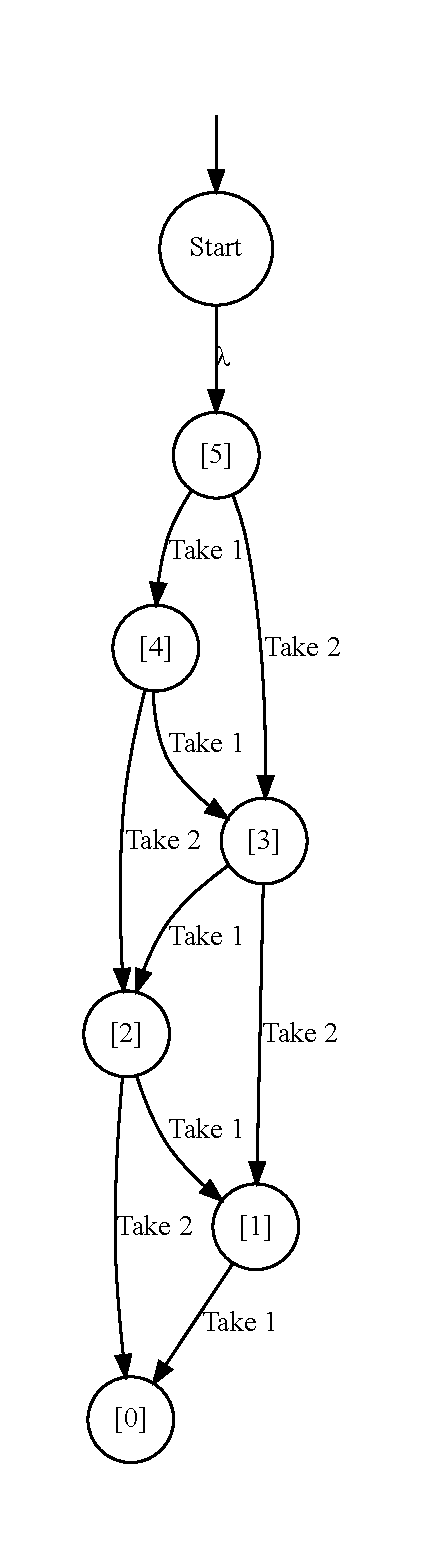
\includegraphics[width=0.55\linewidth]{figures/nimexample/heapFSM.pdf}
    \caption{The Heap finite state machine.}
    \label{fig:nimHeapFSM} 
\end{figure}

We prefer to process the inputs as (A,2), (B,1), and (A,2), so that the player making the move and the number of subtracted tokens are processed in lock step.  In this way, any actions associated with each move will be properly taken upon that move.  Similarly, if the game had 3~heaps in play instead of a single heap, we want all heaps to be modified by each turn.  Concatenation focuses on one heap until it is exhausted before moving to the next heap.   Finally, consider that the first machine accepts~ABAB which would be inappropriate if the second machine accepts~212, since only~3 moves are made.  The lock-step execution we require is over inputs for each machine that are the same length.

\begin{figure}
    \centering
    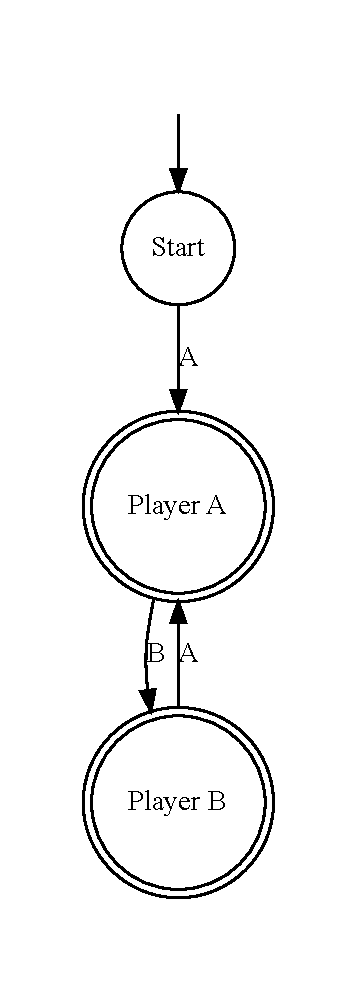
\includegraphics[width=0.35\linewidth]{figures/nimexample/playerFSM.pdf}
    \caption{The Player finite state machine.}
    \label{fig:nimPlayerFSM}
\end{figure}

In support of the semantic actions occurring as they should, and requiring inputs of the same length, we present in Section~\ref{sec:cpalg} an algorithm for constructing a particular \emph{cross product} of two FSMs.  For our example here, the resulting FSM is shown in Figure~\ref{fig:nimFSM}.  The cross product of the two machines nicely distinguishes a win by~A from a win by~B, and clearly a move and its player are processed in lock step.

\begin{figure}
    \centering
    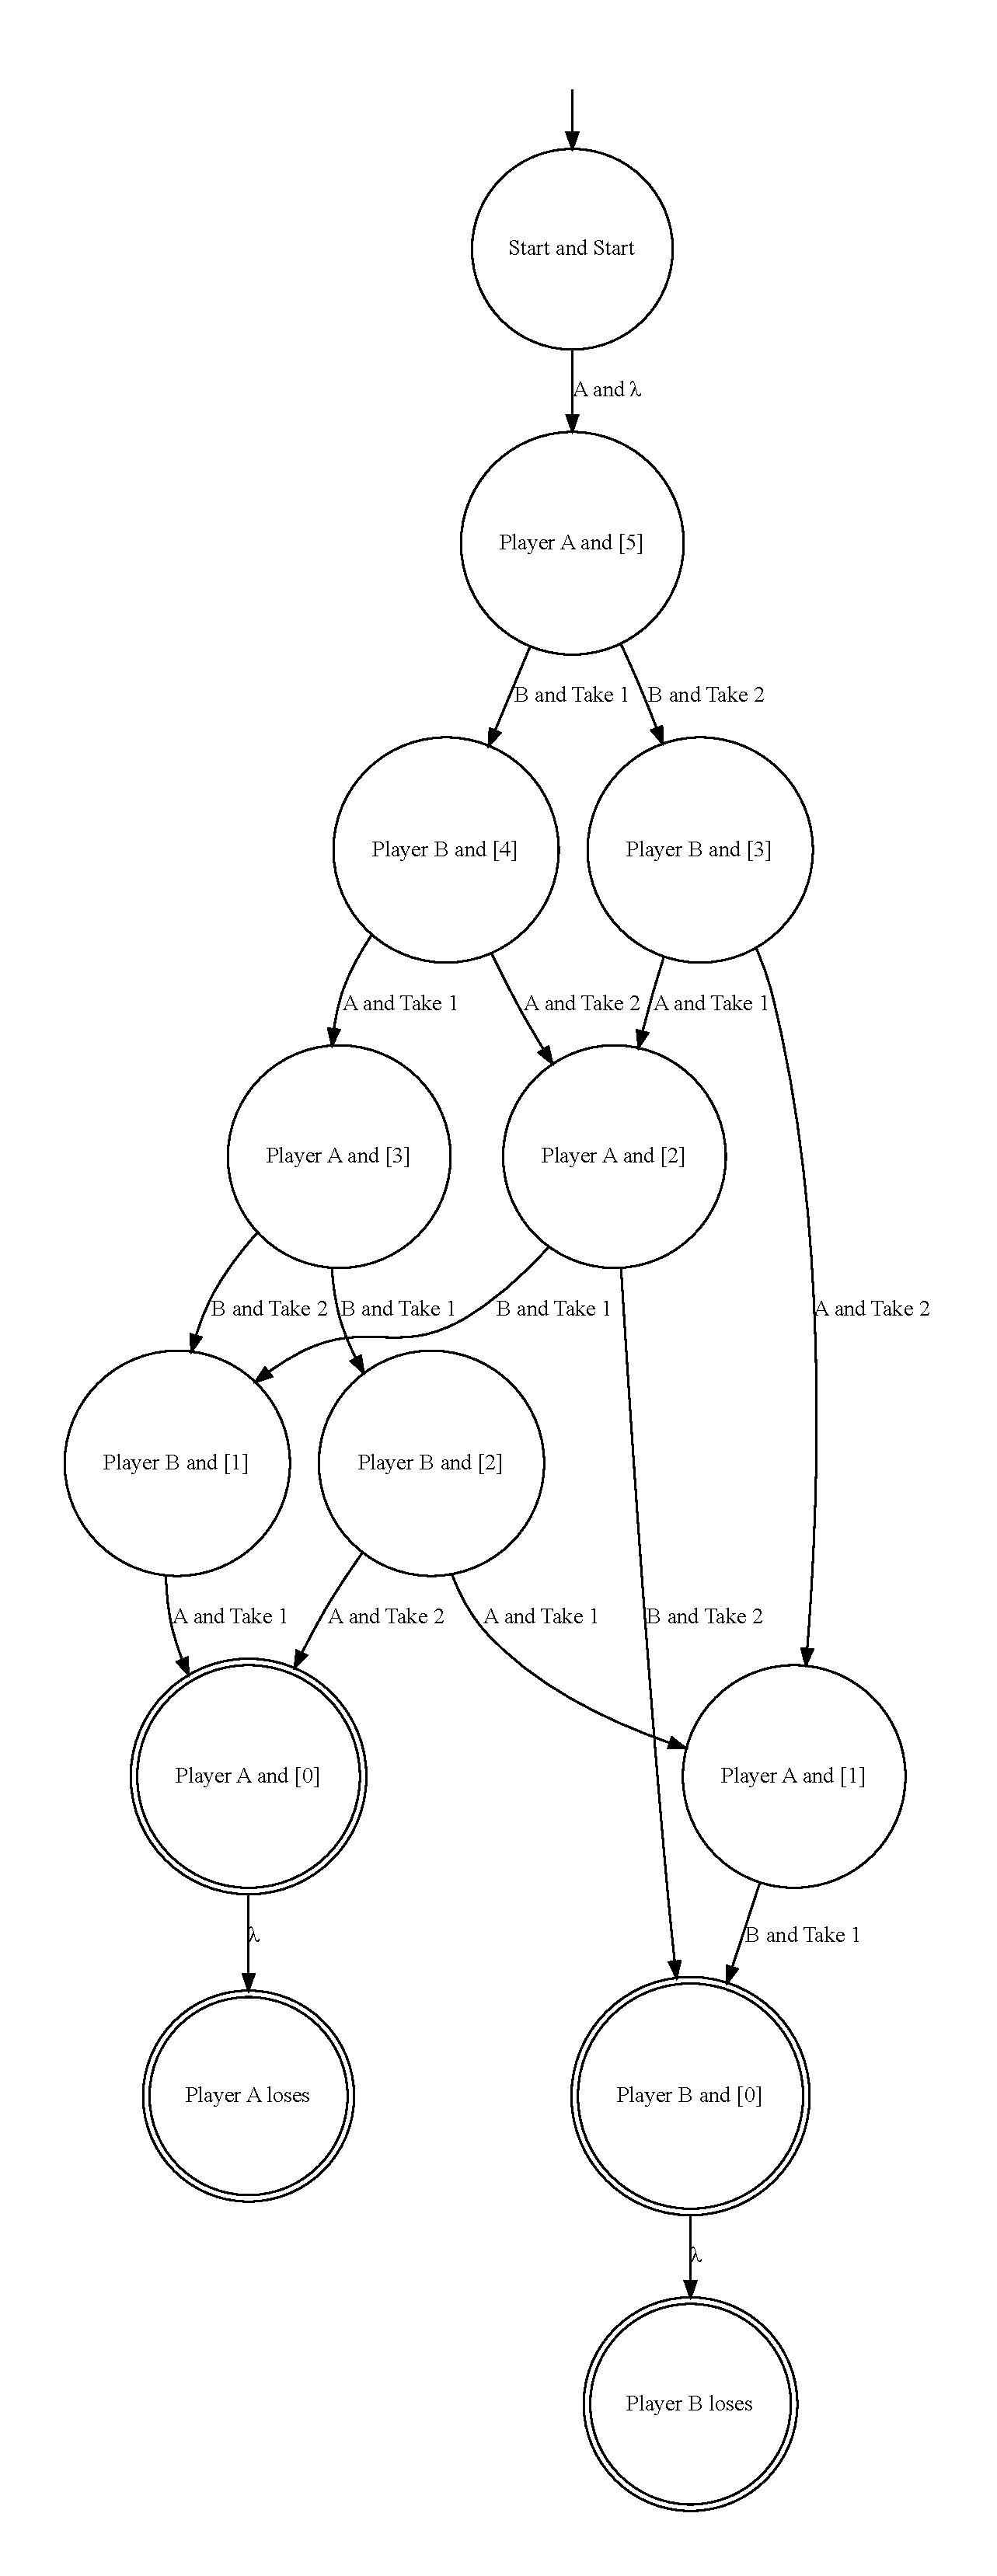
\includegraphics[width=0.6\linewidth]{figures/nimexample/nimFSM.pdf}
    \caption{The resulting Nim finite state machine.}
    \label{fig:nimFSM}
\end{figure}

\section{Formalism}\label{sec:formal}
We have developed a formalism to describe both of the feature-decomposition techniques. We begin with an FSM $M$, typically defined as follows: 
\[M = (Q, \Sigma, \delta, q_0, F)\]where $Q$ is a set of states, $\Sigma$ is a set of input symbols, $\delta$ is the transition function, $q_0$ is the start state, and $F$ is the set of accepting states.  A state is typically denoted by an upper-case letter;  lower-case letters denote input symbols and strings.  The symbol $\lambda$ denotes the empty string.  When an FSM is drawn as a graph, the start state receives an edge with no sources, and an accepting state is drawn with two concentric circles. 

The formalisms presented here are implemented in Chisel as a library we call Foam, described in Section~\ref{sec:foam}.  The examples and results presented in this paper were created using Foam.  

\subsection{Cross-cutting features}
We follow~\cite{aspectsUML} in the treatment of aspects for FSMs.  Essentially a state is like a method and a transition between states is like a method call.  The usual forms of before, after, and around advice are available (\textit{cf}. AspectJ~\cite{AspectJ:01}).   A cross-cutting feature is implemented using advice that modifies an FSMs behavior before, after or during a transition between states.

% A path through an FSM can be described as a sequence of alternating states and input tokens. The FSM in Figure~\ref{fig:example} contains two paths from the start to accept state: $XxYyZ$ and $XtZ$. 
As described below, a feature is comprised of \emph{advice} applied to \emph{pointcuts} of an FSM, which can formally change the language of the machine, but more broadly the advice can affect actions taken by the machine as its input is processed.  

\begin{figure}
    \centering
    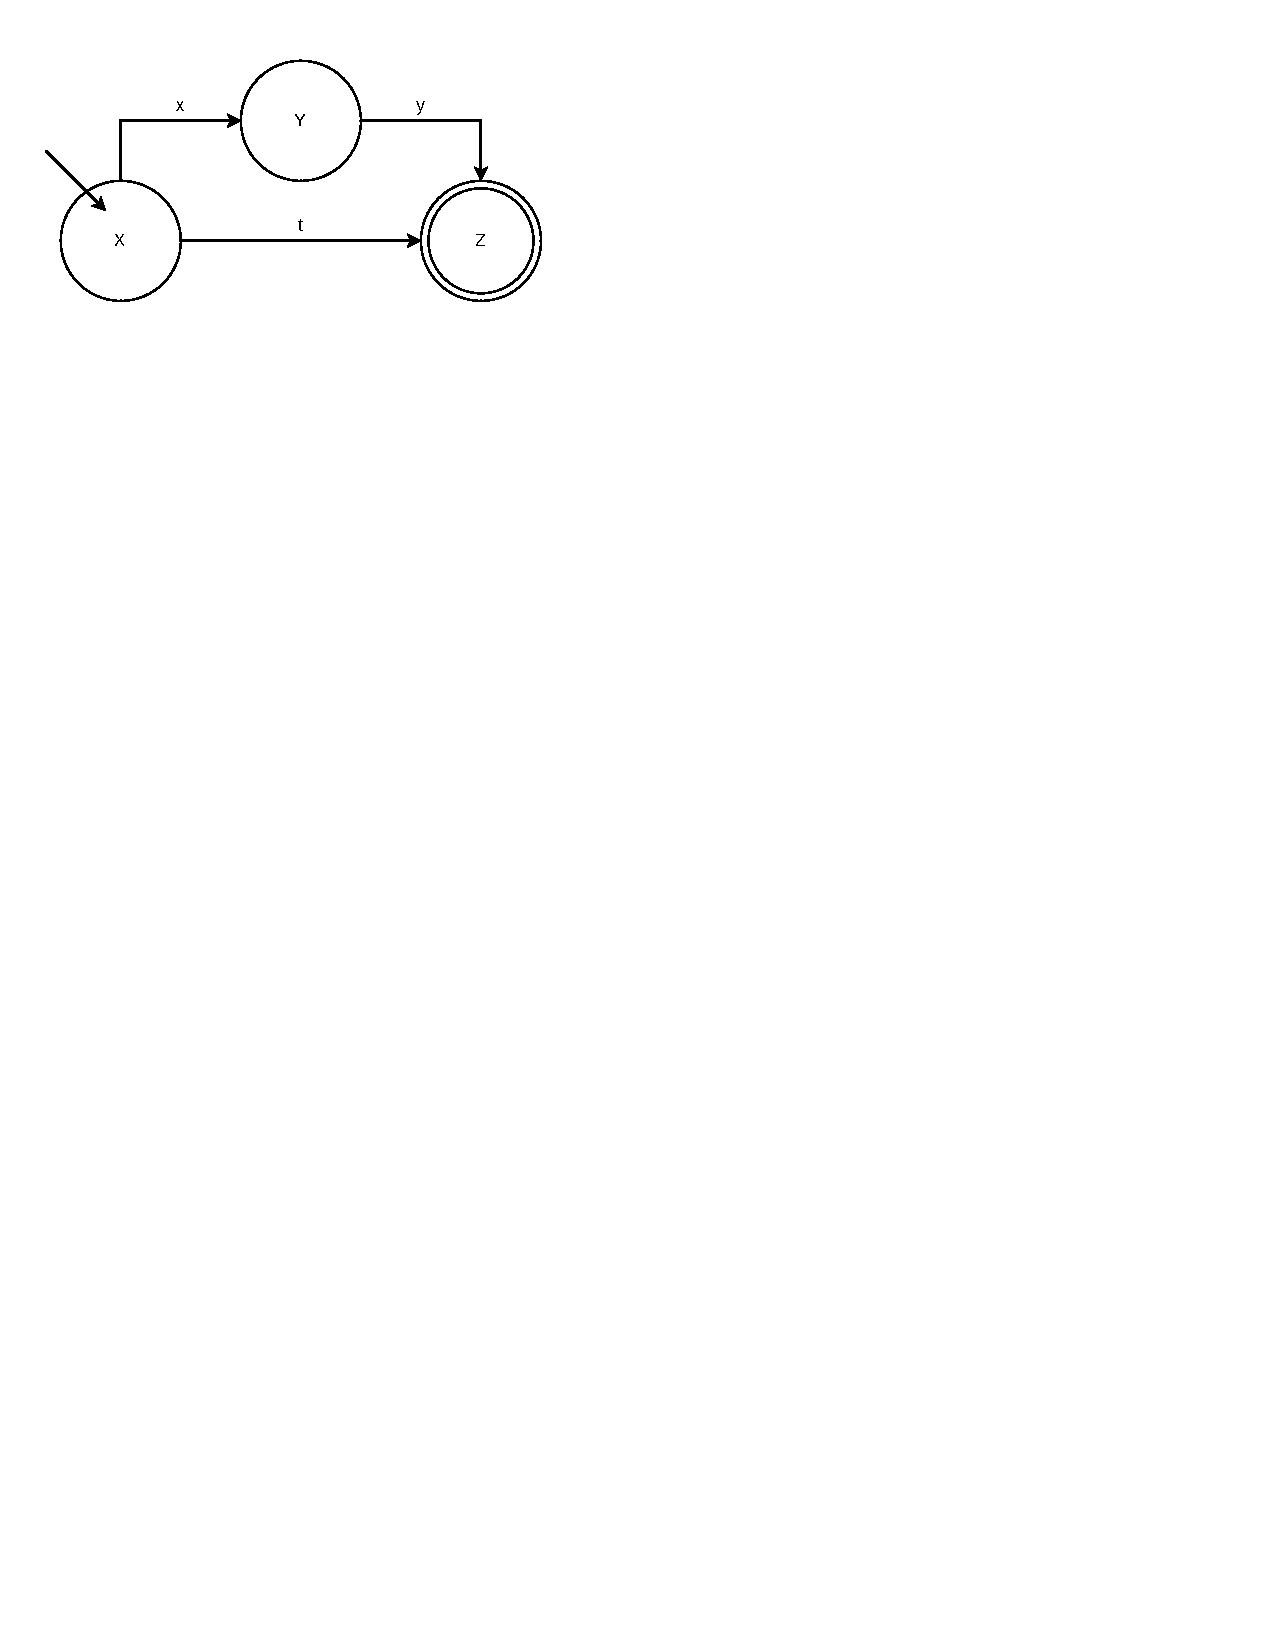
\includegraphics[width=0.7\linewidth]{figures/ExampleFSM.pdf}
    \caption{FSM to illustrate application of peanut-warning advice.  The transition on $t$ is not yet processed, but the transition on $x$ now includes a warning in state~$Y$.}
    \label{fig:applyadvice}
\end{figure}

\paragraph{Pointcuts} These specify \emph{where} advice should be applied in a targeted FSM.   The generative nature of Chisel removes the need for new syntax to express pointcuts.  Instead, we can select states, transitions, or symbols using simple set quantifiers and predicates, written in Chisel/Scala and executed along with the rest of Chisel code that generates a circuit.  For example, a peanut-allergy warning can be generated in a vending-machine FSM through \emph{before} advice applied to any node that would vend a product containing peanuts.  Such properties are implemented nicely in Scala using \emph{traits}.  To implement this feature, the base code likely requires refactoring to include the peanuts trait.  However, the effort is worthwhile because the refactoring and associated advice make the resulting product both clearer and more easily able to exclude or include actions taken on vending products with peanuts.

In AOP terminology, a pointcut yields a set of \emph{joinpoints} at which advice is applied.  A joinpoint associated with the above example would be a single state~$Z$ at which a peanut product is vended.  Because this is a \emph{before} pointcut, the joinpoint has context that includes the state~$X$ prior to $Z$ and the action $t$ that causes the transition, as shown in Figure~\ref{fig:applyadvice}.  The result of applying the relevant advice is shown also, if $X$ made a transition on $x$ to $Z$.   The state $Y$ is now introduced to warn of peanuts, and confirmation to proceed is now represented by transition $y$ to $Z$. \rnote{change the figure and letters to make this more meaningful!} 

\rnote{I think this formalism is unnecessary and clouds the examples we need}  As such, a pointcut $\Pi$ is either $\Pi_Q = \{q : q \in Q, C(q) = \mathrm{true}\}$ or $\Pi_\Sigma = \{\sigma : \sigma \in \Sigma, C(\sigma) = \mathrm{true}\}$, where $C$ is some matching criteria such as type.

\paragraph{Advice} This specifies \emph{what} should happen at a joinpoint.  The advice is passed a joinpoint that includes all context for the advice's application.  \rnote{again why do we need this?  Instead talk about the peanut-warning advice} In our formalism, advice $\Delta$ is a function that returns a valid path through the FSM. The set of possible paths is defined as \[\Psi = \{A\alpha: A \in Q, \alpha \in \Sigma\} \cup \{\beta B: \beta \in \Sigma, B \in Q\} \cup Q \cup \Sigma.
\] So, $\Delta_Q: \Pi_Q \rightarrow \Psi$ and $\Delta_\Sigma: \Pi_\Sigma \rightarrow \Psi$.The pattern of the required path depends on where in the FSM the pointcut is making modifications. Since a state may have multiple paths go through it or an input token may be used in multiple paths, $\Delta$ is not only parameterized with the join-point $p$, but also information about the path it is being applied to. Advice in our system is \emph{context aware}, meaning that $\Delta$ can return different paths depending upon the path under consideration. 

For simplicity, we introduce three sets of path information $\Theta, \Omega$, and $\Gamma$ defined as:
\begin{align*}
    \Theta &= \{A \alpha | \forall p \in \Pi_Q, \exists A \in Q, \exists \alpha \in \Sigma \text{ s.t. } p \in \delta(A, \alpha)\}\\
    \Omega &= \{\beta B | \forall p \in \Pi_Q, \exists \beta \in \Sigma, \exists B \in Q \text{ s.t. } p \in \delta(\beta, B)\}\\
    \Gamma &= \{AB | \forall p \in \Pi_\Sigma, \exists A \in Q, \exists B \in Q \text {s.t. } B \in \delta(A, p)\}
\end{align*}

$\Theta$ and $\Gamma$ capture all the immediate paths that the state join-point $p$ is involved in. Whereas, $\Gamma$ captures the paths that the transition join-point $p$ is involved in. 

\subsubsection{State Features}
We can now express the three types of advice application for states in terms of $\Pi, \Delta, \Theta$, and $\Omega$.\\
\textbf{Before:} $\forall p \in \Pi \ \forall A \alpha \in \Theta \quad A \alpha p \rightarrow A \alpha \Delta(p, A \alpha)p$\\
\textbf{After:} $\forall p \in \Pi \ \forall \beta B \in \Omega \quad p\beta B \rightarrow P\Delta(p, \beta B)\beta B$\\
\textbf{Around:} \\
$\forall p \in \Pi \ \forall A \alpha \in \Theta \ \forall \beta B \in \Omega \quad A \alpha p \beta B \rightarrow A \alpha \Delta(p, A \alpha, B \beta) \beta B $

\paragraph{Buy More} As an example, let's consider the \textbf{Buy More} feature. After each time the machine dispenses a product (represented in the system as a \texttt{DispenseState}) the machine should transition back to a state where the total value in the machine represents product price subtracted from the original value in the machine (represented as a \texttt{TotalState}).

\begin{align*}
C: Q &\rightarrow \{\mathrm{true},\mathrm{false}\}\\
q &\mapsto q.\text{type} = \text{DispenseState} \\
\Pi_Q &= \{q: q \in Q, C(q) = true\}\\
\Delta_Q &: \Pi_Q \times \Psi \rightarrow \Psi\\
(q, \psi) &\rightarrow \lambda[\text{TotalState(funds)}] \\
\text{where funds} &= q.\text{product.value} - q.\text{value}
\end{align*}
This $\Delta_Q$ is applied using the after method. Figure \ref{fig:vend2} shows the application of this feature on the vending machine FSM from Figure \ref{fig:vend1}. Note, the \texttt{DispenseState} has been split by another feature used in the construction of \textbf{Buy More} to preserve value information and construct the correct path.

\begin{figure*}
    \centering
    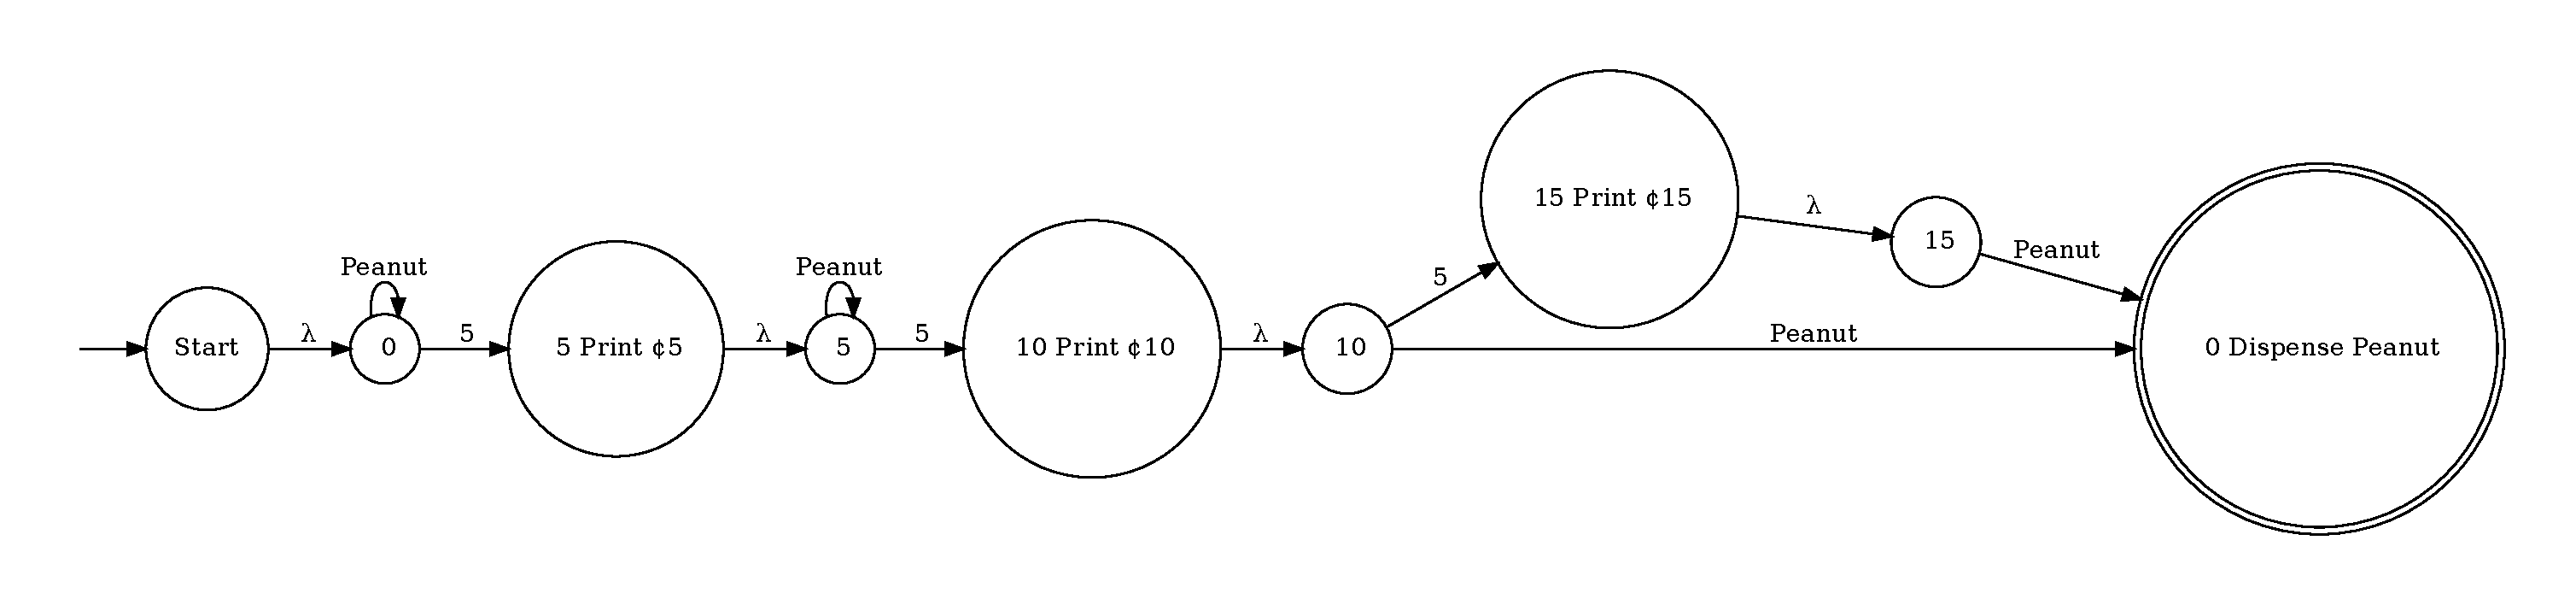
\includegraphics[width=0.7\textwidth]{figures/vend2.pdf}
    \caption{The resulting FSM of the application of Buy More to the FSM from Figure \ref{fig:vend1}.}
    \label{fig:vend2}
\end{figure*}

\subsubsection{Transition Features}
Similarly, we can express the three types of advice application for input tokens in terms of $\Pi, \Delta$, and $\Gamma$.\\
\textbf{Before:} $\forall p \in \Pi \ \forall AB \in \Gamma \quad A p B \rightarrow A \Delta(p, A, B)pB$\\
\textbf{After:} $\forall p \in \Pi \ \forall AB \in \Gamma \quad A p B \rightarrow A p \Delta(p, A, B)B$\\
\textbf{Around:} $\forall p \in \Pi \ \forall AB \in \Gamma \quad A p B \rightarrow A  \Delta(p, A, B)B$

\paragraph{Print Funds} For an example of applying advice to an input token, let's consider the \textbf{Print Funds} feature. Here, after each transition on a piece of currency, the machine should print out the new total value. Note, here we need to check the value of $B$ to make sure that we do not reapply the same advice again.

\begin{align*}
C: \Sigma &\rightarrow \{\mathrm{true},\mathrm{false}\}\\
\sigma &\mapsto \sigma.\text{type} = \text{CurrencyToken} \\
\Pi_\Sigma &= \{\sigma: \sigma \in \Sigma, C(\sigma) = \mathrm{true}\}\\
\Delta_\Sigma &: \Pi_\Sigma \times \Psi \rightarrow \Psi\\
(\sigma, \psi) &\rightarrow \begin{cases}
    \emptyset & \text{if newState} = \sigma\\
    \text{newState}, \lambda & \text{else}\\
\end{cases}\\
\text{where newState} &= \text{PrinterState}(\psi.B.\text{value})
\end{align*}
This $\Delta_\Sigma$ is applied using the after method. As above, Figure \ref{fig:vend3} shows the resulting FSM after the application of the \textbf{Print Funds} feature. This is a kin to the logging example from Section \ref{sec:prior}.

\begin{figure*}
    \centering
    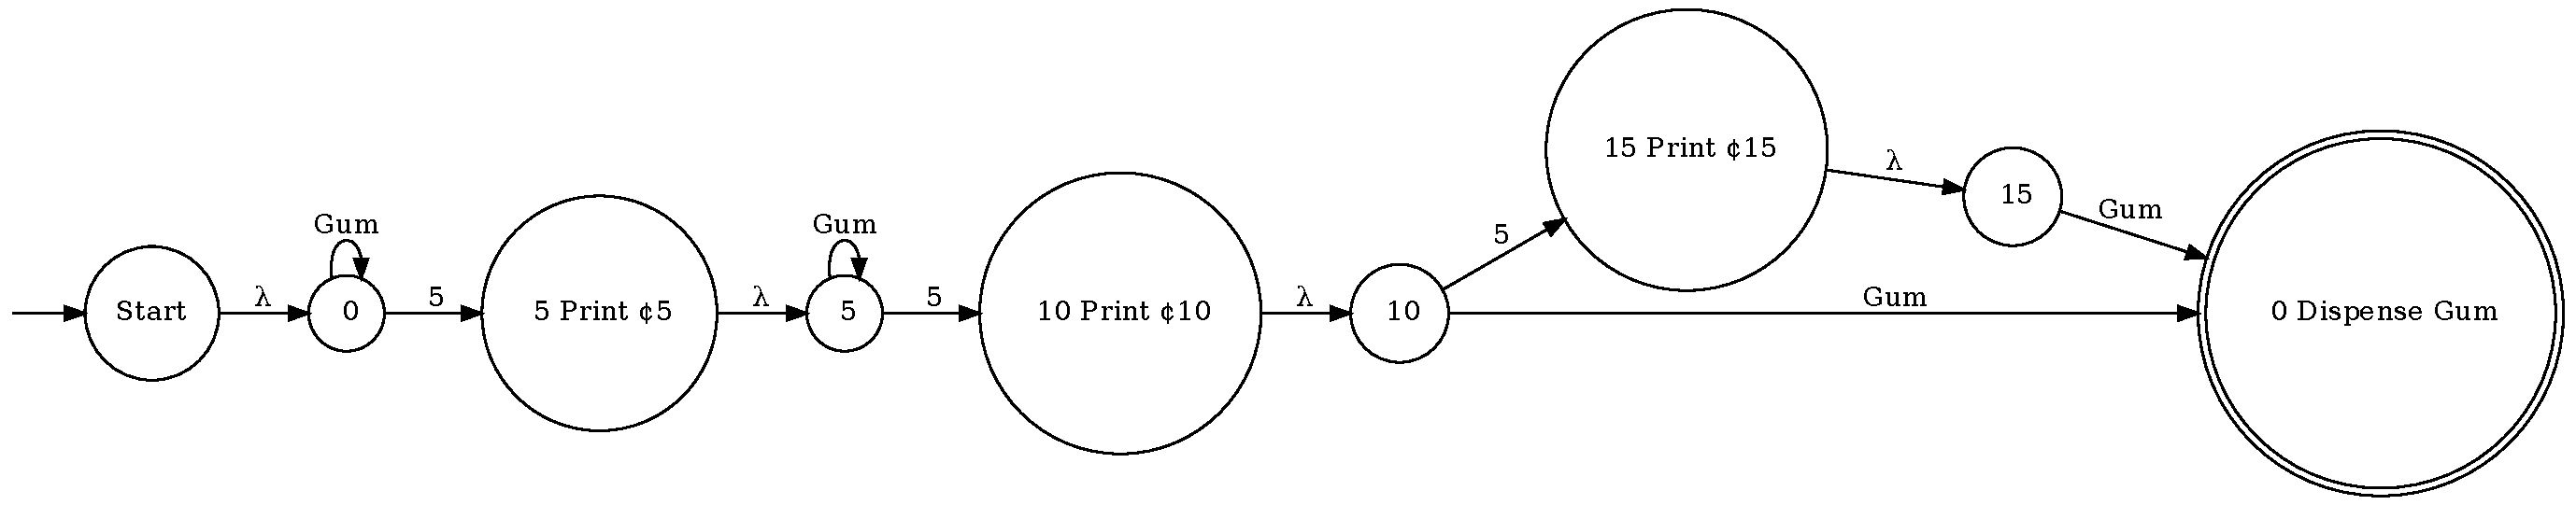
\includegraphics[width=0.8\textwidth]{figures/vend3.pdf}
    \caption{The resulting FSM of the application of Print Funds to the FSM from Figure \ref{fig:vend3}.}
    \label{fig:vend3}
\end{figure*}

\subsection{Cross Product Features}\label{sec:cpalg}
\todo{This section}
\pnote{Do we provide motivation here? E.g., how this is different from the union/intersection machine constructs, and how this is fundamentally different from the concatenation machine?}
\pnote{Where should we reference Sipser's proof of regular languages being closed under union?}

\begin{algorithm}
\caption{Cross Product Machine}

\begin{algorithmic}[1]
\REQUIRE {$M_1 = (Q_1, \Sigma_1, \delta_1, q_{01}, F_1), M_2 = (Q_2, \Sigma_2, \delta_2, q_{02}, F_2)$}
\ENSURE {$M = (Q, \Sigma, \delta, q_0, F)$}
    \STATE {$q_0 \gets (q_{01}, q_{02})$}
    \STATE {$Q \gets \{q_0\}$}
    \STATE {$\Sigma \gets \emptyset$}
    \STATE {$\forall q \in Q_1 \times Q_2, \forall a \in \Sigma_1 \times \Sigma_2, \delta(q, a) \gets \emptyset$}
    \STATE {$\delta' \gets \delta$} \COMMENT{This is used to determine when to stop iterating.}
    \REPEAT
        \STATE{$\delta' \gets \delta$}
        \FOR{$\mathbf{q} = (q_1, q_2) \in Q$}
            \STATE{$\mathrm{M_1Trans} \gets \{ (a_1, r_1) : \forall a_1 \in \Sigma_1, \delta_1(q_1, a_1) = r_1 \}$}
            \STATE{$\mathrm{M_2Trans} \gets \{ (a_2, r_2) : \forall a_2 \in \Sigma_2, \delta_2(q_2, a_2) = r_2 \}$}
            
            \FOR{$((a_1, r_1), (a_2, r_2)) \in \mathrm{M_1Trans} \times \mathrm{M_2Trans}$}
                \STATE{$\mathbf{r} \gets (r_1, r_2)$} 
                \STATE{$\mathbf{\sigma} \gets (a_1, a_2)$} 
                \STATE{$Q \gets Q \cup \mathbf{r}$}
                \STATE{$\Sigma \gets \Sigma \cup \mathbf{\sigma}$}
                \STATE{$\delta(\mathbf{q}, \sigma) \gets \delta(\mathbf{q}, \sigma) \cup \mathbf{r}$}
                
                \IF{$r_1 \in F_1 \land r_2 \in F_2$}
                    \STATE{$F \gets F \cup \mathbf{r}$}
                \ENDIF
            \ENDFOR
        \ENDFOR
    \UNTIL{$\delta = \delta'$}
\end{algorithmic}
\end{algorithm}

Let $M_1 = (Q_1, \Sigma_1, \delta_1, q_{01}, F_1)$ and $M_2 = (Q_2, \Sigma_2, \delta_2, q_{02}, F_2)$ be finite state machines. Then we may construct the cross product machine, $M = M_1 \times M_2 = (Q, \Sigma, \delta, q_0, F)$ as: 

\begin{enumerate}
    \item $Q = Q_1 \times Q_2$
    \item $\Sigma = \Sigma_1 \times \Sigma_2$
    \item $q_0 = (q_{01}, q_{02})$
    \item $F = (F_1 \times Q_2) \cap (Q_1 \times F_2)$
    \item Define $\delta$ such that $\forall \mathbf{r} = (r_1, r_2) \in Q, \forall \mathbf{a} = (a_1, a_2) \in \Sigma,$ 
\end{enumerate}
\[\delta(\mathbf r, \mathbf a) = \begin{cases}
    (\delta_1(r_1, a_1), \delta_2(r_2, a_2)) & \delta_i(r_i, a_i) \neq \emptyset, i = 1, 2\\
    \emptyset & \mathrm{else}
\end{cases}\]

\section{Aspect Oriented Finite State Machine Library}\label{sec:foam}
We have implemented an aspect oriented finite state machine library, which we call Foam,  in Scala\footnote{https://github.com/wustl-frisc/foam}. In this section, we detail the library as well as code generation.

While Foam is not a fully fledged domain specific language, we have modeled the interface after the well established aspect-oriented extension to Java, AspectJ~\cite{}. The intention is to give aspect-oriented practitioners a familiar interface for interacting with the finite state machines. Since the library is implemented in plain Scala, we have access to and utilize the full powers of the type system. Following our vending machine example, Figure~\ref{lst:PrintFunds} shows the implementation of the \textbf{Print Funds} feature in Foam.

We provide a series of extendable base classes to represent finite state machines. The library takes care of building pointcuts, applying aspects, and performing the cross-product. We have even provided reflexive access, just like AspectJ to the join-point and its incoming and outgoing paths. Given this, in relatively few lines of code, programmers can create advice with ease.

\begin{figure*}
    \centering
    \begin{lstlisting}[language = Scala]
class PrintFunds extends Aspect[NFA] {
  def apply(nfa: NFA) = {

    val tokenPointcut = Pointcutter[Token, Coin](nfa.alphabet, token => token match {
      case t: Coin => true
      case _ => false
    })

    AfterToken[Coin](tokenPointcut, nfa)((thisJoinpoint: TokenJoinpoint[Coin], thisNFA: NFA) => {
      var value = thisJoinpoint.out.asInstanceOf[ValueState].value
      thisJoinpoint.out match {
        case s: PrinterState if (s.action == "Funds:" + value.toString) => (None, thisNFA)
        case _ => (Some((PrinterState("Funds:" + value, value, false), Lambda)), thisNFA)
      }
    })
  }
}
\end{lstlisting}
    \caption{The implementation of the PrintFunds feature in Foam.}
    \label{lst:PrintFunds}
\end{figure*}

\subsection{Code Generation}
The library currently supports emitting GraphVis and Verilog code. Code generation is decoupled from the creation of the finite state machines, as the library generates code based off the internal data structures, not the Scala code itself. Code GraphVis and Verilog code are generated by Graphviz4S~\cite{} and Chisel, respectively. 

\section{Case Studies}
Here we present three case studies to demonstrate the generative ability of our framework: a Vending Machine, the game of Nim, and SIMD cache coherence.

\subsection{Vending Machine}
We implemented all the features from Section \ref{sec:vend} in our library. The resulting FSMs were then emitted as Verilog. The Verilog was then synthesized on a xc7a35tcpg236-1 FPGA using Vivado 2022.1. Below we report the number of generated states, transitions in the FSM, and the space in LUTs that the FSM took up in on the FPGA.

Figure \ref{fig:vmData} shows the results for different endpoints generated by our library. For our tests, we held the currency threshold at 100. Every machine contains 5, 10, 25 value coins and 4 products of value 25, 50, 75, and 100. This is captured by \textit{None}. In the first set of results, each feature is shown by itself. Even single features can greatly increase the components in the FSM. The \textbf{Buy More} feature (denoted B) by itself more than doubles the number of states and transitions. This impressive leverage is further exemplified when combining features. 

In these cases the number of states increase by 2.5x in the simplest endpoint up to 4.6x in the most complex, and the transitions by 2.5x and 5x respectively. Recall, this is in a relatively simple vending machine that can only accept up to 100 units of value. Simply doubling the amount of accepted value to 200 creates a machine with 284 states (10.5x increase over the base) and 3113 transitions (16x increase over the base). However, this is accomplished in our library with relatively few lines of code. The largest feature in terms of code is \textbf{Peanut Warning}, which is implemented in just 39 lines. \jnote{Report the lines of code for each feature?}

Despite the huge number of generated states and transitions, the resulting LUTs taken up by the FSM are linear. This is due to the fact that hardware synthesis tools can encode the states using a linear scheme. However, the original specification of that circuit \textit{must be expressed in the exponential form first} for the synthesis tools to recognize it. With our framework, hardware designers are not limited to small finite state machines.

\begin{figure}
    \centering
\begin{tabular}{lrrrr}\toprule
Features &States &Transitions &LUTs \\\midrule
None &27 &208 &24 \\
P &47 &368 &38 \\
I &47 &368 &46 \\
C &48 &423 &70 \\
W &33 &320 &60 \\
B &57 &448 &60 \\
PI &67 &528 &73 \\
PICB &118 &1053 &186 \\
PICW &94 &1023 &160 \\
PICWB &124 &1353 &220 \\
\bottomrule
\end{tabular}
    \caption{Number of generated states, transitions, and LUTs depending on selected features. The features are as follows: P = Print Funds, I = Insufficient Funds, C = Change Return, W = Peanut Warning, and B = Buy More.}
    \label{fig:vmData}
\end{figure}

\subsection{Nim}\label{sec:nim}
\todo{Removed ``tokens'' from the data.}
\paragraph{Traditional Nim}
The classical game of Nim is a mis\`{e}re game of two players and a finite number of heaps. Each turn, the current player may only remove tokens from a single heap of their choosing, and must take between 1 and all the tokens remaining in that heap. 

In the simplest variation of traditional Nim, with a single heap containing three tokens and only allowing one player, six states and five tokens were created, as seen in Figure~\ref{tab:traditionalNim}. However, the results quickly explode as the number of players increase, and predominately, as the number of heaps and their initial quantities of tokens increases. Allowing for three heaps, containing 3, 4, and 5 tokens respectively, and having two players -- a common example used to introduce Nim -- already contains 235 states, 26 tokens, and 6110 transitions. 

\begin{figure}
\small
\begin{tabular}{rrrrrrrr}\toprule
\multicolumn{3}{c}{Heaps} &Players &States &Tokens &Transitions \\\cmidrule{1-7}
3 &4 &5 & & & & \\\midrule
\checkmark & & &1 &6 &5 &30 \\
\checkmark & & &2 &9 &7 &63 \\
\checkmark & & &4 &11 &8 &88 \\
\checkmark &\checkmark & &1 &22 &9 &198 \\
\checkmark &\checkmark & &2 &39 &16 &624 \\
\checkmark &\checkmark & &4 &60 &30 &1800 \\
\checkmark & \checkmark &\checkmark &1 &112 &14 &1708 \\
\checkmark & \checkmark &\checkmark &2 &235 &26 &6110 \\
\checkmark & \checkmark &\checkmark &4 &419 &50 &20950 \\
\bottomrule
\end{tabular}
\caption{Number of generated states, tokens, and transitions by selected features for traditional Nim. Each game was played as Mis\`{e}re play.}\label{tab:traditionalNim}
\end{figure}

\paragraph{The Subtraction Game}
The Subtraction game is a single heap variation of Nim, usually played by a small group of players. The players take turns in a round-robin style and remove between one and a pre-determined number of tokens. As the game is played as a Mis\`{e}re game, the player taking the final token loses. 

\begin{figure}
\small
\begin{tabular}{cccrrrrr}\toprule
\multicolumn{3}{c}{Allowed} & & & & \\
\multicolumn{3}{c}{Moves} &Players &States &Tokens &Transitions \\\cmidrule{1-7}
-1 &-2 &-3 & & & & \\\midrule
\checkmark & & &1 &24 &3 &72 \\
\checkmark & & &2 &24 &4 &96 \\
\checkmark & & &4 &24 &6 &144 \\
\checkmark &\checkmark & &1 &24 &4 &96 \\
\checkmark &\checkmark & &2 &45 &6 &270 \\
\checkmark &\checkmark & &4 &81 &10 &810 \\
\checkmark & \checkmark &\checkmark &1 &24 &5 &120 \\
\checkmark & \checkmark &\checkmark &2 &45 &8 &360 \\
\checkmark & \checkmark &\checkmark &4 &83 &14 &1162 \\
\bottomrule
\end{tabular}
\caption{Number of generated states, tokens, and transitions for the Subtraction game. Every game is played with a single starting heap of 21 tokens and through Mis\`{e}re play. }\label{tab:subtractionNim}
\end{figure}

\paragraph{Circle Nim}
Circle Nim is a variation of Nim where the heaps are placed around a circle. Each turn, players are allowed to take tokens from between one and an upper-bounded quantity of consecutive heaps, taking between one and every token within each heap. This is often played as a mis\`{e}re game. 

\begin{figure}
\small
\begin{tabular}{cccrrr}\toprule
Heaps &Players &States &Tokens &Transitions \\\midrule
3 &1 &10 &11 &110 \\
3 &2 &15 &17 &255 \\
3 &4 &17 &20 &340 \\
6 &1 &66 &20 &1320 \\
6 &2 &113 &38 &4294 \\
6 &4 &150 &74 &11100 \\
9 &1 &514 &29 &14906 \\
9 &2 &951 &56 &53256 \\
9 &4 &1429 &110 &157190 \\
\bottomrule
\end{tabular}
\caption{Number of generated states, tokens, and transitions by variation of features for Circle Nim. Each heap contained one token, players could take between one and three consecutive tokens, and all games were played as Mis\`{e}re play. }\label{tab:circleNim}
\end{figure}

\subsection{SIMD Caches}\label{sec:cache}
Ultimately, the goal of this work is to make the design of complex hardware easier through generation. Here, we will demonstrate how we can combine our techniques with ``off the shelf'' components to generate SIMD Caches that are coherent with each other. While we recognize that this is purely a pedagogical example, it is modeled off the real-world RDNA Architecture from AMD~\cite{}.

\paragraph{RDNA Architecture} The RDNA architecture packages two SIMD execution units into a single unit called a \textit{work-group processors}. Each work-group shares L0 cache between each SIMD unit. This cache is kept coherent through serialization of the execution when conflicts are detected. Two work-groups are then packaged together into a \textit{Dual Compute Unit} (DCU). Currently, the two L0s within a DCU are kept coherent via software. At the beginning of each clock cycle, four separate instructions are issued to each of the SIMD units from the L0 instruction cache.

Suppose that we wanted to recreate this cache system ourselves, but instead keep the L0s coherent using the MSI cache coherence protocol~\cite{}. To begin, we have selected the ready-made cache from RISC-V Mini~\cite{}. As-is, this cache, shown in Figure \ref{fig:cacheBefore}, is directly connected to main memory in a single core system and does not have any coherence protocol. Using a feature oriented approach, we can retrofit this cache with advice that implements the MSI protocol, shown in Figure \ref{fig:cacheAfter}. We can then instantiate and cross-product the number of cache FSMs we need to govern the whole process. 

\begin{figure}
    \centering
    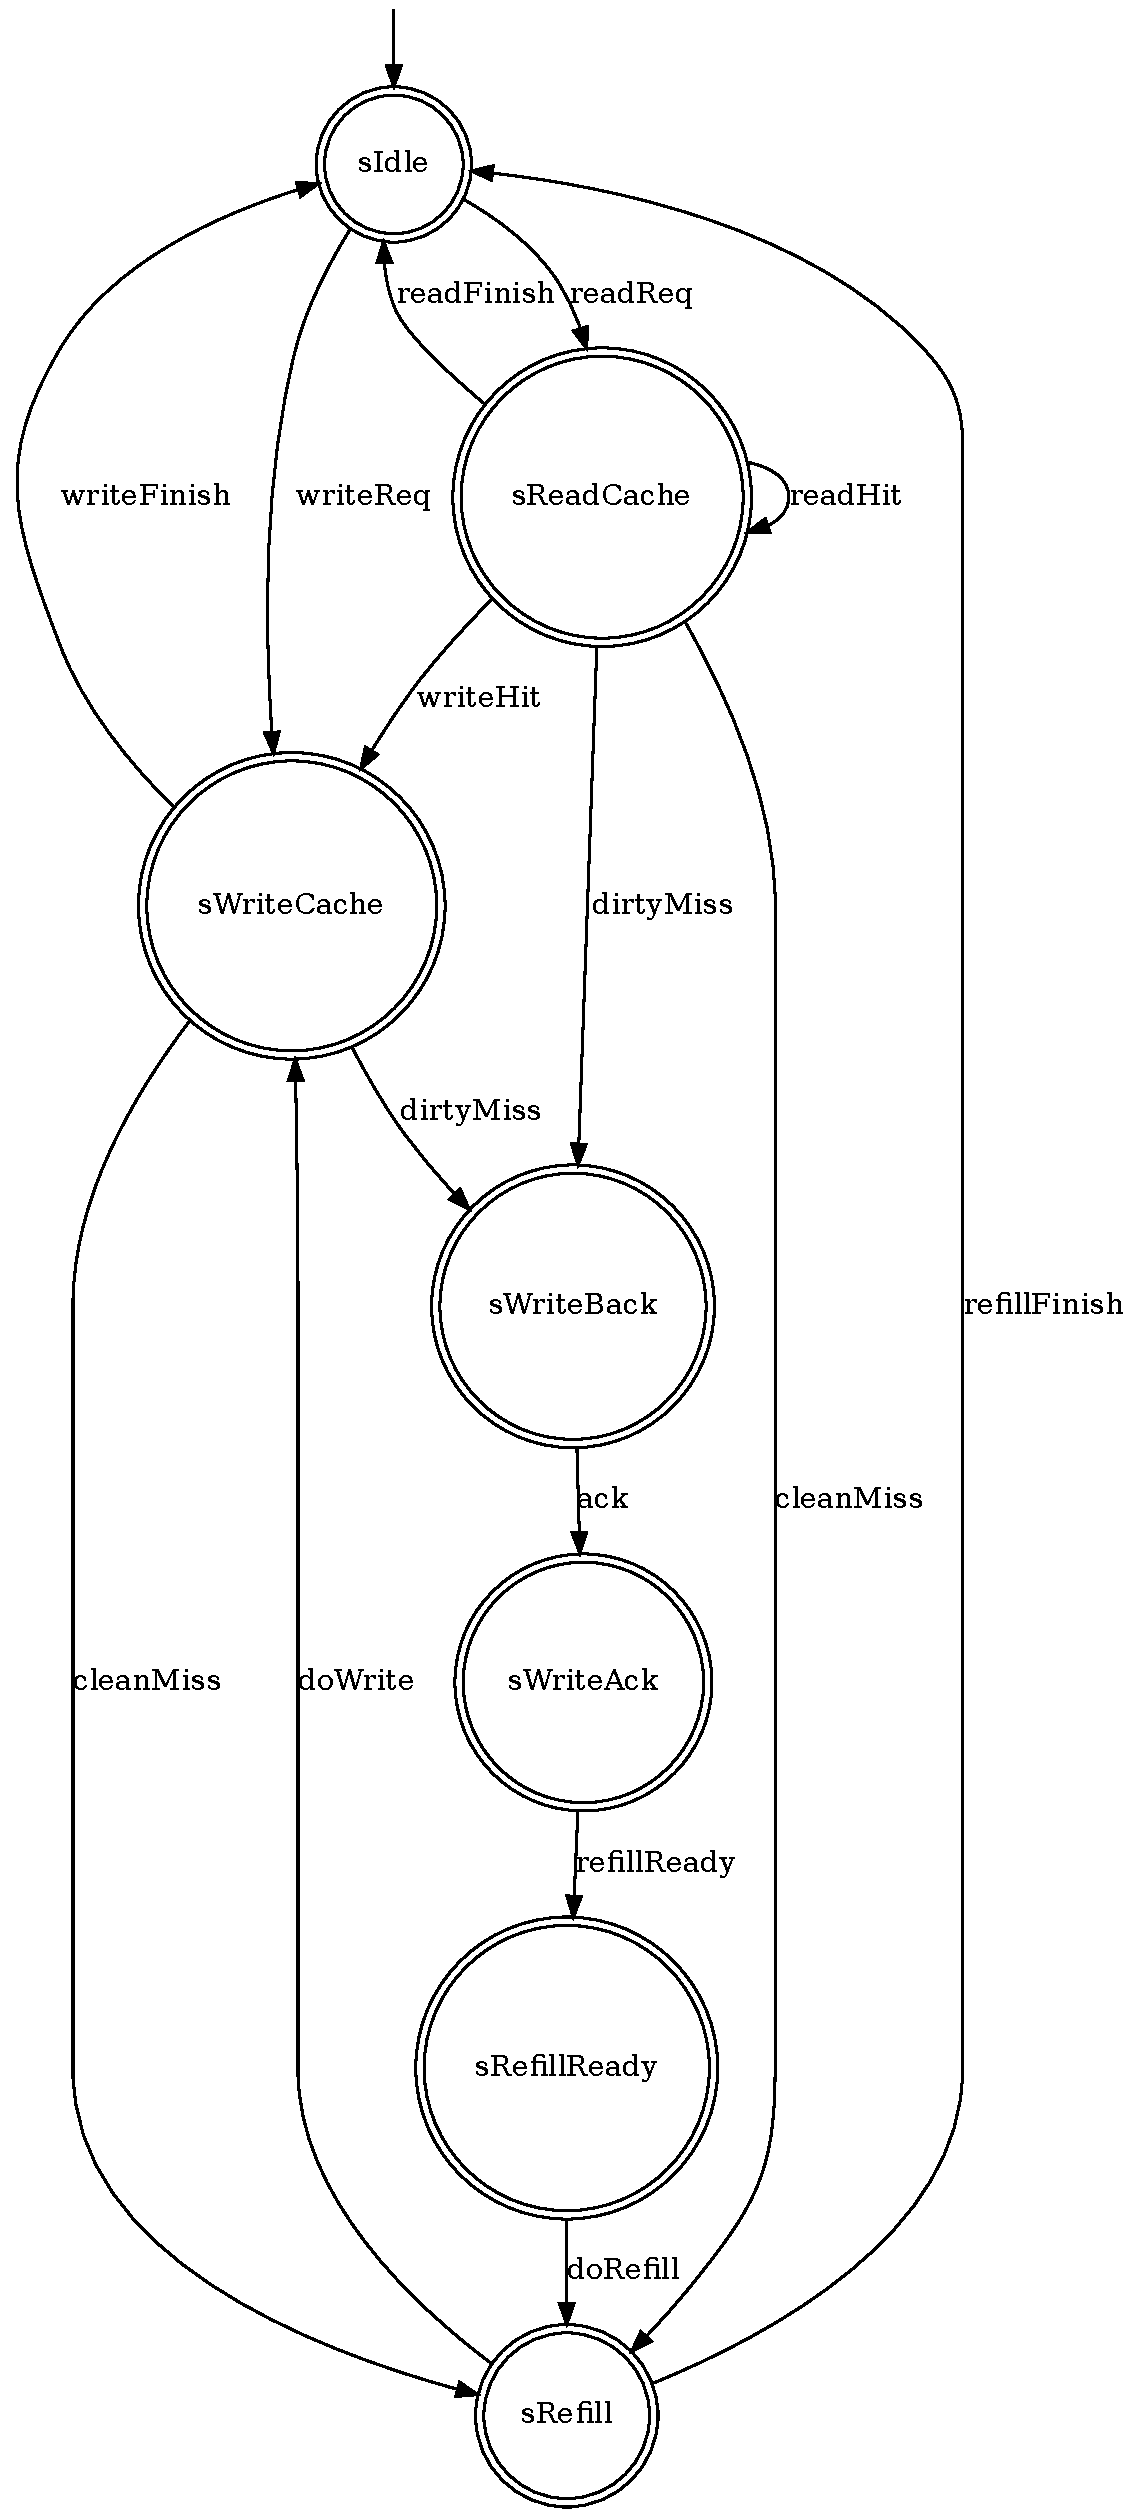
\includegraphics[width=0.7\linewidth]{figures/cacheFSM.pdf}
    \caption{The cache FSM from the RISC-V Mini.}
    \label{fig:cacheBefore}
\end{figure}

\begin{figure}
    \centering
    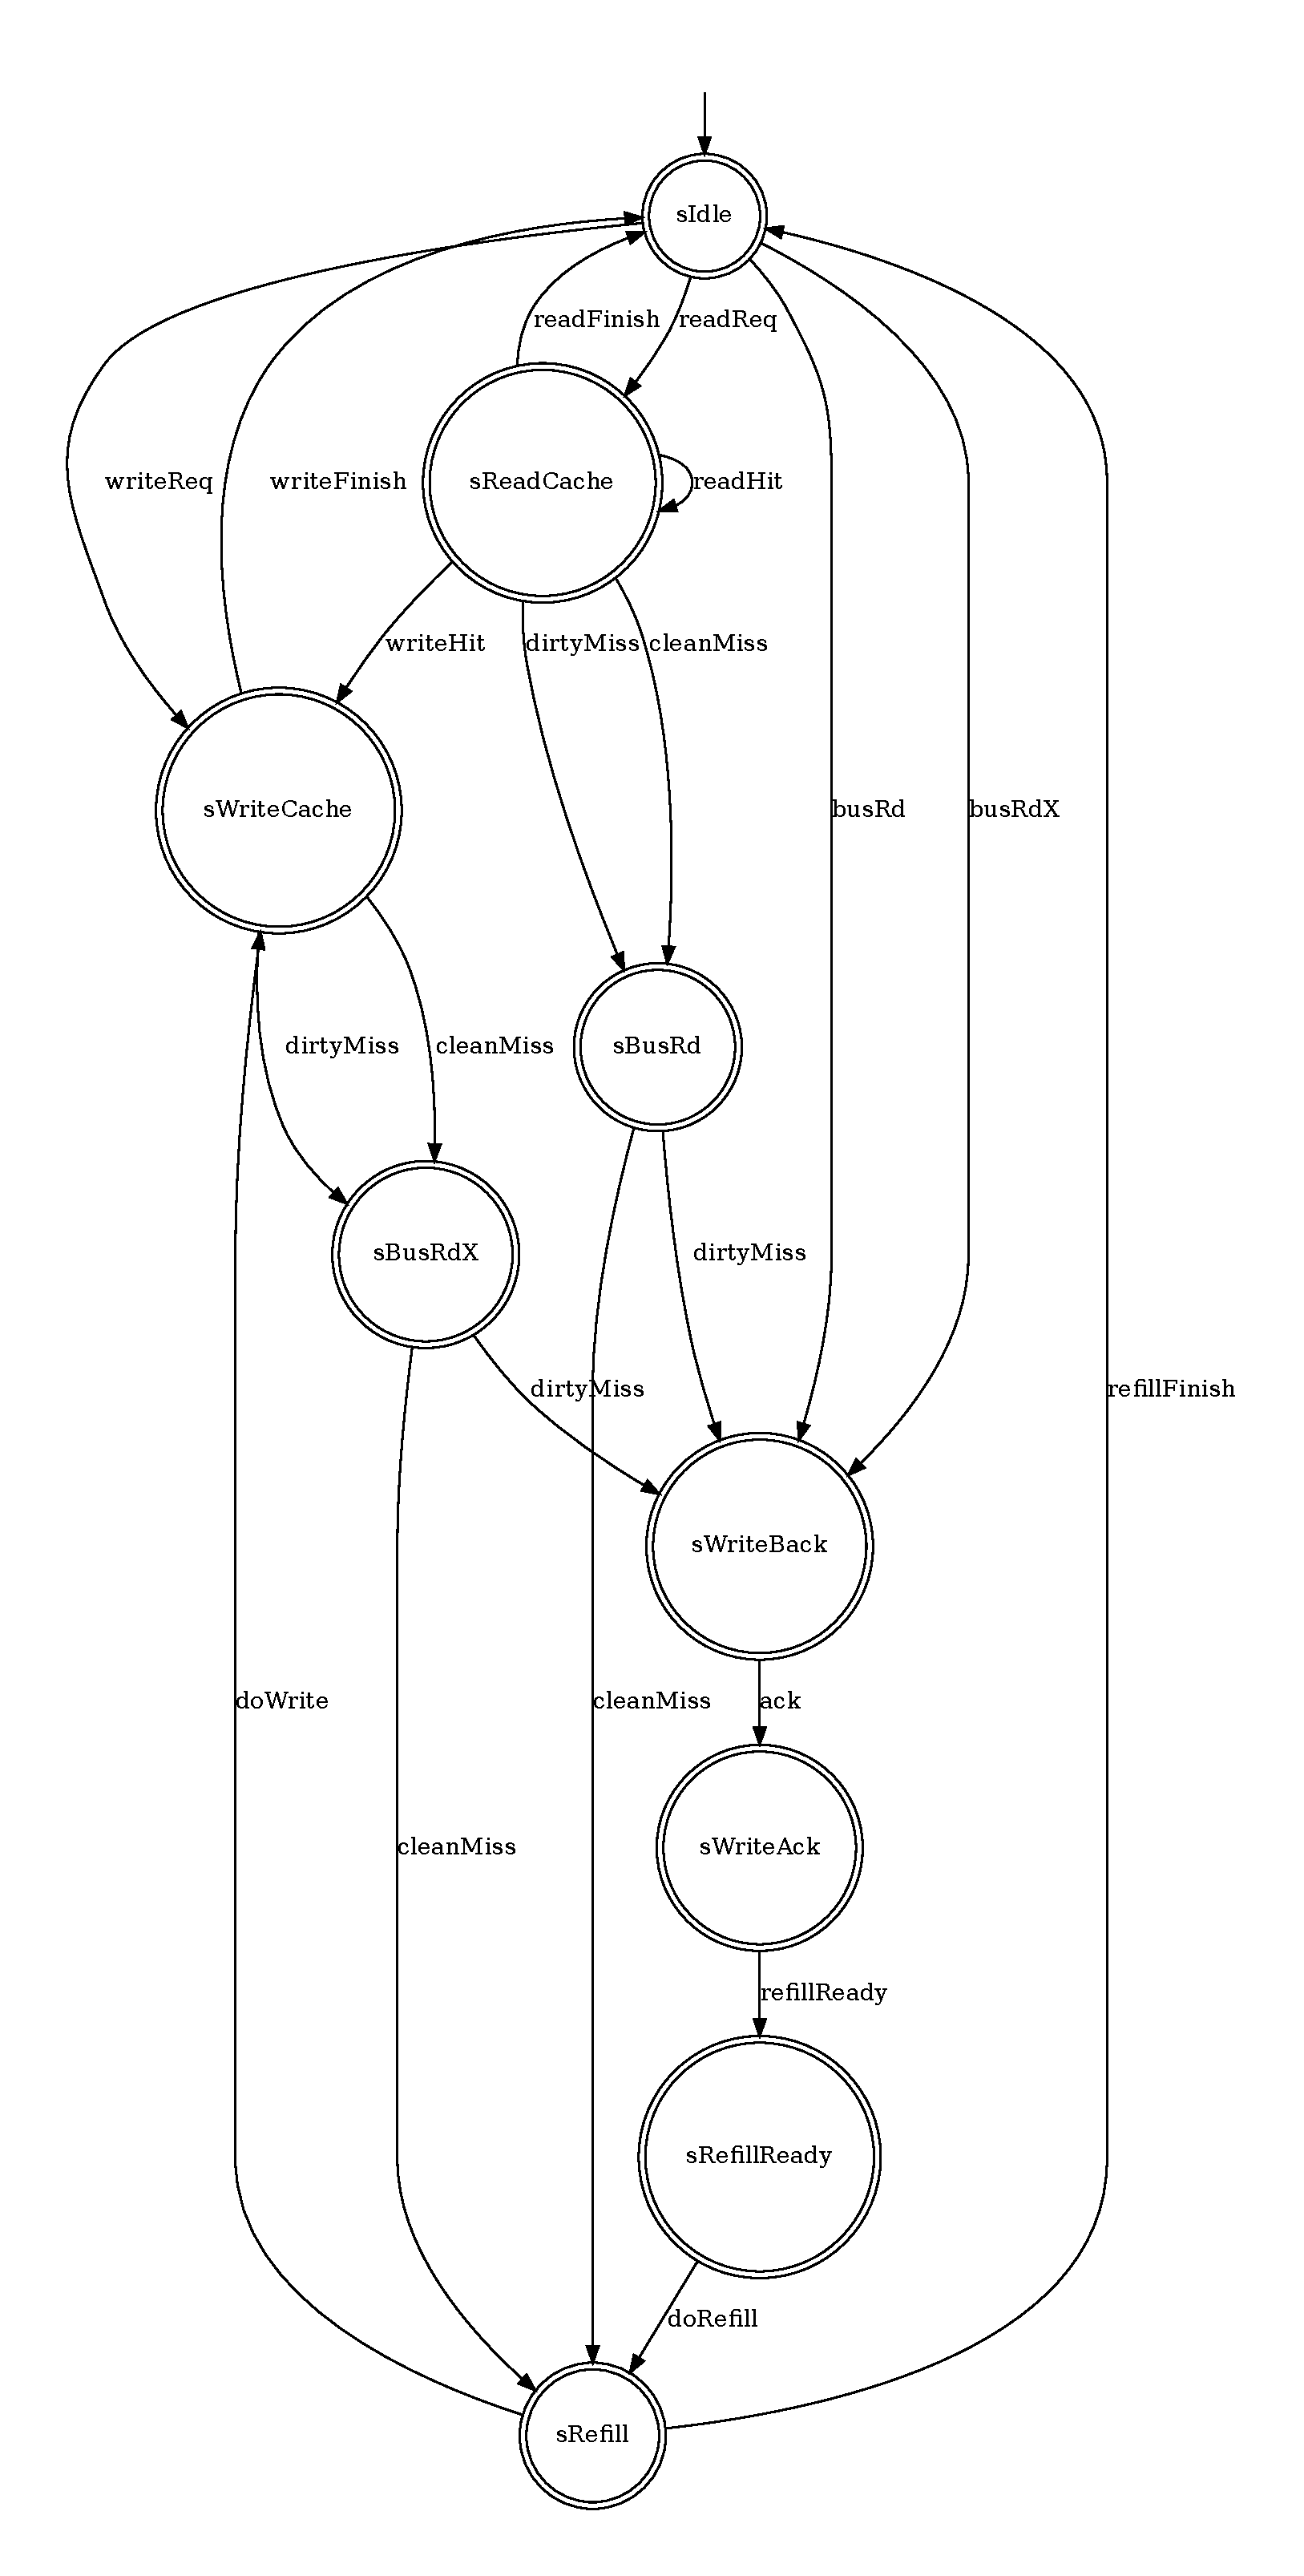
\includegraphics[width=0.7\linewidth]{figures/cacheFSM2.pdf}
    \caption{The cache FSM from RISC-V Mini with the MSI protocol.}
    \label{fig:cacheAfter}
\end{figure}

While hardware designers may not choose to have a single FSM govern all cache interactions in actuality, this technique is still extremely useful for modeling the interactions between the caches. Imagine that in the next iteration of the architecture, the ``Dual Compute Unit'' becomes a ``Quad Compute Unit''. Instead of having to start completely from scratch, hardware designers can simply instantiate two more caches into the system. Furthermore, instead of being locked into a single cache coherence protocol, the hardware designers may want to choose the MESI protocol~\cite{}, for their next iteration. With our approach, this protocol can just be applied instead of the MSI protocol. This requires zero direct refactoring on the FSM itself.

\jnote{Talk about how we can show the original language accepted by the cache is a subset of the new language --> there's no surprises vis-a-vis cpu communication.}

\section{Future Work}
\jnote{Call back to Cache, explain how with a FO-cache we could model RDNA even closer... write through, 4-way, LRU policy}

%%
%% The next two lines define the bibliography style to be used, and
%% the bibliography file.
\bibliographystyle{ACM-Reference-Format}
\bibliography{acmart,bibdbase,networks}

\end{document}
\endinput
%%
%% End of file `sample-sigplan.tex'.
